\chapter{Build the System}\label{chapter:build}

In the next chapter, a detail description of the process of the system development following the methodology introduced before and how the methodology was adapted and implemented are presented. 

\section{Acquiring Context Relevance} \label{sec:acr}

The first step of the methodology is to discover the relevance of the contextual factors to the current implementation domain (i.e. clothes shopping). 

To adapt the recommendations to the user's current contextual situation requires an understanding of the relationship between user preferences and contextual conditions. Thus it is proposed that explicit user ratings or any form of preferences should be given under several different contextual conditions. For instance, the user must rate a given clothes item when the temperature is hot, warm and cold. It is quite time and resource consuming because the user needs to only give ratings after they have experienced the context. Therefore, to reduce the risk of collecting data for unimportant context factors, an experiment needs to be first set up to determine which context factors are interesting to study \cite{ref:18}. 

The experiment should be able to investigate how the influence of each contextual factors changes on user's purchasing decision for different clothes types and to provide quantitative measurements so that they can be used as weight in the similarity measurement in the following retrieving algorithm. Considering all above reasons, the methodology developed in paper \cite{ref:18} was adopted to assess the context relevance.

This methodology is based on a web tool for acquiring context relevance judgements and a statistical data analysis method to quantitatively measure the influence of each contextual conditions on different clothes types. Following this methodology, a web survey was designed and developed in this thesis. First, an initial set of contextual factors and conditions (values for the factors) were selected referring to some existing literatures about context-aware applications \cite{ref:5, ref:12, ref:19}. The selected contextual factors and conditions are listed in Table \ref{tab:factors}. Then, the clothes items were retrieved from Zalando \footnote{http://www.zalando.co.uk/}. Especially, clothes of these brands are collected: Marc O'Polo, Tom Tailor, Esprit, S.Oliver, Benetton. Because these five brands are in the middle price category and are well known and generally acceptable by most people. Moreover, the types and number of clothes offered by these brands are similar to each other and are rich enough to cover most common clothes types. After the clothes were retrieved, they were aggregated into a relatively small list of categories so that the problem of data sparseness can be avoided. Totally, 14 categories were defined: tops, dresses, underwear, cardigans, trousers, coats, blouses, jackets, skirts, jeans, socks, swimwear, suits and shirts.

\begin{table}[H]
	\centering
	\caption{Context factors used in the Web survey}
	\label{tab:factors}
	\begin{tabular}{p{1.1in}p{1.6in}|p{1.1in}p{1.6in}} \hline
		Context Factor & Conditions  & Context Factor & Conditions  \\ \hline 
		budget & budget buyer & purchasing intent & work \\
 		& high spender &  & daily wear \\
 		& price-for-quality buyer &  & party \\
		time of the day & morning time &  & sports \\
 		& afternoon &  & no special \\
 		& night time & companion & with girl-/boy-friend \\
		day of the week & weekend &  & with family  \\
		& working day &  & with children \\
		crowdedness & shop is crowded &  & alone \\
		& shop is not crowded &  & with friends \\
		& shop is empty & weather  & snowing \\
		mood & shopaholic &  & clear sky \\
		& outdoorsy &  & sunny \\
		& like a party animal &  & raining \\
		& normal &  & cloudy \\	
		season & spring & transport & walking \\
 		& summer &  & public transport \\
 		& autumn &  & bicycle \\
 		& winter &  & car \\
		temperature & warm & time available & half day \\
 		& cold &  & one day \\
 		& hot \\ \hline
	\end{tabular}
\end{table}


After the data was prepared, a simple web application was developed for acquiring the relevance of the selected contextual factors for different clothes categories (see Figure \ref{fig:webtool}). In the web application,users are randomly given a clothes category and are asked to imagine themselves being under a randomly chosen contextual condition and then choose the influence of the selected contextual condition on their intentions to buy the selected type of clothes. As an example of the questions posed to the user consider the situation depicted in Figure \ref{fig:webtool}. Here we first requested the user to imagine a typical shopping scenario: "Imagine that you are in Munich and you are doing offline shopping for clothes. You are thinking about buying Skirts." Then the user was asked to select the influence (i.e., positive, no effect, negative) of the three randomly chosen contextual conditions on their decision to buy the clothes. As an example of a contextual condition: "Imagine that the weather is cloudy." Every user was requested to interact with at least 10 of these pages (as in Figure \ref{fig:webtool}). 

\begin{figure}[H]
	\centering
	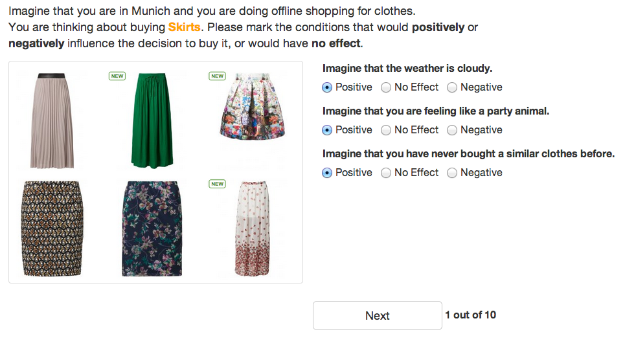
\includegraphics[height=2.8in]{figures/webtool.png}
	\caption{Web based survey tool to acquire context relevance.}
	\label{fig:webtool}
\end{figure}



38 participants took part in this web survey. Overall 1190 responses were given to one of the questions shown in Figure \ref{fig:webtool}. Because no pre-knowledge was known whether certain context conditions are more likely to influence user's decision, we sampled the value of clothes categories and contextual conditions using uniform distribution so that all possible values can be reached with equal opportunities.

\subsection{Analysis of Context Relevance} \label{sec:acr_acr}

The goal of this web survey in this thesis is to find out quantitatively how the context factors influence user decisions on whether or not to buy clothes from different categories. 

The web survey delivered samples for the distribution $P(I|C_i,T)$ where $I$ (Influence) is the response variable taking one of the three values: positive, negative, or no effect, $T$ is a clothes category (e.g., tops, skirts), and $C_1, ... C_N$ are the context factors that may or may not influence the user decision. This distribution models the influence of the context factors on the user's purchasing decision considering different clothes categories. 

The spread of a categorical variable $X={x_1, ... x_n}$ can be measured by looking at the entropy of the random variable \cite{ref:45}. If $P(X=x_i)=\pi_i$, the entropy of $X$ is: 
$$E(X)=-\sum_{1\leq i\leq n}\pi_i \cdot log{\pi_i} $$

This measurement of the spread can be used to estimate the association between variable $X_1$:  user's intention to buy a certain item (i.e., positive, negative or no effect) and variable $X_2$: one of the current context factor (e.g., current budget). Informally, if the influence of the context factor is strong, then the spread of variable $X_1$ will be reduced if $X_2$ is known, and it is weak if the spread of $X_1$ remains unchanged even if $X_2$ is known and this association can be formally defined as \cite{ref:18}:
$$U=\frac{E(X_1)-\mathcal{E}(E(X_1|X_2))}{E(X_1)}$$
where $E(X_1)-\mathcal{E}(E(X_1|X_2))$ is the difference between the spread of $X_1$ and the expected spread of $X_2$ which measures the influence of the context factor to user's decision. $\mathcal{E}(X)$ denotes the expected value of the random variable $X$. $U$ is 1 if the spread of $(X_1|X_2)$ is zero. $U$ is zero, however, if $X_2$ does not have any influence of $X_1$. U can be seen as the mutual information of $X_1$ and $X_2$ normalized to the interval [0,1]. 

With the definition, $U$ can be used to measure how good $I$ - the influence of context on the user's purchasing decision - can be predicted if $C_i$ - one of the relevant context factors - is known \cite{ref:18}. In this thesis, the computed $U$ of each context factors for all clothes types was computed and used as weight factor for similarity assessment. The ordered context factors in descending order of $U$ for each clothes category can be seen in Appendix \ref{appendix:upcc} of this paper.

\section{The Proposed Approach} \label{sec:pa}

This section describes the recommendation approach that was built. The goal of this approach is to integrate the contextual information into the recommendation process and recommend items that might be of interest to users under a specific context situation.

To integrate the contextual information into the recommender system,  context-driven querying and search approach was adopted. As was introduced in Section \ref{sec:rs_cars_rci}, this approach uses contextual information and/or user's specified interest to query or search a repository of resources and presents the most appropriate ones to the user. The repository usually contains resources that are tagged with contextual information while collecting them. Corresponding to this approach, case-based recommendation technique was used to realize it. As was discussed in Section \ref{sec:rs_cbrs}, case-based recommendation technique is a branch of knowledge-based recommendation. Compared to collaborative filtering and content-based techniques, case-based recommendation has no cold-start problem because it can rely on the case base (or knowledge base) for the initial recommendation. This case base can be set up quickly using expert experience and does not require pre-training like what was done in paper \cite{ref:5} for model-based approach. 

Each case in the case base is composed of an item and the contextual situation under which the item is bought. Here a contextual situation is a combination of several context factors and their corresponding values. For example, the user may ask for recommendation of clothes for work (condition one) when the weather is warm (condition two). For the recommendation, the user first submits the contextual information as a query. Then the system searches in the case base and selects the cases with the most similar context situation and then recommends the items or items similar to the items contained in the retrieved cases to the user. 

On the other hand, knowledge-based recommender system has the disadvantage of static suggestion ability because the knowledge-base is usually preset by domain experts and barely changes. Also usually the domain experts and the knowledge engineers are not the same person, the communication cost requires an efficient way for knowledge engineering. Based on those considerations, in this thesis the case-based recommendation approach was extended by integrating collaborative filtering approach for case base (knowledge base) setup so that all the application users can play the expert role and their purchased items together with the contextual information can be added to the case base as a new case for future recommendation. Although the collaborative filtering approach was used, the correlation between users was performed at the session level (i.e., each submitted case is independent of itself and will not be related to the user who submits the case). Thus no user identification is required and a considerable amount of example data is not needed for each single user in order to deliver effective recommendations \cite{ref:26}.

\section{Towards Case-Based Recommender System} \label{sec:tcbrs}

As was introduced in section \ref{sec:rs_cbrs}, case-based recommender systems apply case-based reasoning (CBR) methodology to solve recommendation problems by re-using or adapting past recommendation solutions stored in past similar cases. In the CBRSs framework introduced in paper \cite{ref:22}, a typical recommendation process is composed of six steps: retrieval, reuse, revise, review, retain and iterate. This framework was used to build the context-aware case-based recommender system in this thesis and will be explained step by step below.

\textbf{Input}: To get a list of recommendations, the user first submits a query of current contextual information. A query is composed of a logical query with fixed context constraints and a feature value vector of context factors and their corresponding value that the user wishes to be considered in the recommendation. For example, if a user is a budget buyer and wants to buy clothes for sports purpose when the temperature is hot and the user wants to find clothes items sold in stores that will be still open in the next 30 minutes within 2000 meters, the query will be structured as follows:
\begin{equation} \label{eq:query}
\begin{split}
	query =  \{((distance \leq 2000m)\wedge(timeopen = now+30min)), &\\
	              (budget (budget\; buyer), intent (sports), temperature (hot))\} &
\end{split}
\end{equation}

\textbf{Retrieval}: After the user submits a contextual query, contextual factors such as budget and intent will be used to find and rank cases with similar context. The definition of similarity and the similarity assessment algorithm will be introduced in section \ref{sec:sa}. 

\textbf{Reuse}: In the final recommendation, nine items in the cases are recommended to the user. However those items are not only ranked according to the level of similarity to the current context. As for initial recommendation of conversational recommendation system in an exploratory mobile scenario, diversity is an important consideration to ensure the coverage of the current scope of candidate items. Thus the bounded greedy selection algorithm was extended to select the cases with the most diverse set of items among the retrieved most similar cases. 

\textbf{Revise}: Before the items are recommended to the user, logical constraints such as distance (e.g. find clothes within 2000 meters) or open time (e.g., shops still open in the next 30 minutes) will be used to check the availability of those items. If for example a recommended item is too far away , then other similar items will be recommended instead.

\textbf{Review \& Iterate}: After the initial recommendations are presented, the user can update the recommendations iteratively through critiquing directly on item features. This is also called conversation-based active learning strategy and has been explained in detail in section \cite{sec:rs_alrs}.

\textbf{Retain}: Finally, when the user selects and purchases an item, the time together with the current context situation will be stored as a new case in the case base.

\section{Case Model} \label{sec:cm}

The case base consists of two components: the item bought ($I$) and the context situation ($C$): 
\begin{equation} \label{eq:caseMode}
CB = I \times C
\end{equation}

Each case $c=(i,e) \in CB$ in the case base is composed of two sub-elements $i,e$ which are instances of the spaces $I,C$ respectively. As was introduced before, the cases are not correlated with the user who submits it, thus the user model is not contained in the case in this system. A case is built during a human/machine interaction \cite{ref:26}. In this system , a case is created when the user purchases the item. According to Peak-end Rule introduced in Section \ref{sec:rs_cars_crp}, how a user feels about an experience is highly influenced by the end of the experience. It was assumed here that users give high rates to the items they buy. Since the case is created when the user purchase an item, the evaluation model in the case base was also removed in this system. In the following, these two components will be explained in more detail. 

$C$ is the data structure that defines the context situation under which the item is bought. It is composed of a feature value vector of context factors and their corresponding values that the user wishes to be considered in the recommendation and a feature value vector of context factors and their corresponding factor importance weight. The factor importance weight reflects the level of influence of the context factors to the recommendation of the clothes item contained in the same case. They are determined by the type of the clothes and has been calculated in the experiment introduced in Section \ref{sec:acr}. For a full list of the factor importance weights for different clothes type please see Appendix \ref{appendix:upcc}. The main context factors are: distance, day of the week, temperature, time available, transport, weather, time of the day, crowdedness, intent of purchasing, companion, season and budget. For a detail list of the context factors and their values, please refer to Table \ref{tab:factors}. For a typical example, if a user is a budget buyer and is looking for clothes for sports when the temperature is hot, the context situation can be structured as follows:
\begin{equation} \label{eq:context}
\begin{split}
	{context}_{attributes} = \{(budget (budget\;buyer), intent (sports), temperature (hot)), &\\
	                                            ((w_{budget}(0.7), w_{intent}(0.6), w_{temperature}(0.9))\} &
\end{split}
\end{equation}

$I$ is the data structure that describes the clothes item bought by the user. It is represented as a feature value weight vector \cite{ref:30} and was borrowed directly from the baseline system introduced in Section \ref{sec:rs_bs}. 

With this case model, knowledge of what kind of items users buy in a certain context situation can be obtained. To provide recommendations, cases with context situation similar to the current user's context can be retrieved and the items contained in those cases can be used directly for the recommendation. They can also be used as reference items to find other similar items to recommend. Thus the next section will show how the similarity between the current context and retrieved cases and similarity between items are calculated.

\section{Similarity Assessment} \label{sec:sa}

To get the similarity between the current context and retrieved cases, the Euclidean Overlap Metric (HEOM) was borrowed \cite{ref:26, ref:34}:
\begin{equation} \label{eq:heom}
heom(x,y)=\frac{1}{\sqrt{\sum^n_{i=1}w_i}}\sqrt{\sum^n_{i=1}w_id_i(x_i,y_i)^2}
\end{equation}
where:
\begin{equation}\label{eq:heom_d}
d_i(x_i, y_i)=
\left\{\begin{matrix}
1 & \mbox{if} \; x_i \; \mbox{or} \; y_i \; \mbox{are unknown}\\ 
overlap(x_i,y_i) & \mbox{if the i-th feature is symbolic}\\ 
\frac{|x_i-y_i|}{range_i} & \mbox{if the i-th feature is finite integer or real} 
\end{matrix}\right.
\end{equation}

Here $range_i$ is the difference between the maximum and minimum value of a numeric feature, and $overlap(x_i, y_i)=1$ if $x_i \neq y_i$ and 0 otherwise. This metric measures the distance between two vectors. Thus the further away two vectors, the more similar they are. In this thesis this metric was modified so that it can be applied to the system.

By using the previously discussed case model and query structure, the feature value vectors of context factors describing the context situation in both structures can be fed into the similarity metric. The context factor set contained in user's submitted query is called current context. The context factor set contained in the case is called target context. First, the similarity between current context and target context is calculated for each case. In some cases, the target context may not contain some context factors in the current context specified by the user (e.g., the user enables the context factor shopping intent and budget in current context, but the target context only contains budget). In some other cases, the current context may not contain some context factors contained in the target context. So when computing similarities, user specified context factors are used as base and only the context factors specified by the user in current context are used for similarity assessment. The context factors contained in the target context but not in the current context are ignored, because the user chooses to ignore those factors. If the target context does not contain the context factors specified in current context, the similarity will be added by $1* w_i$. ($w_i$ here corresponds to the feature factor weight).

The simplified similarity metric is displayed as follows:
\begin{algorithm}
\caption{The simplified similarity metric}
\label{list:similarity}
\begin{algorithmic}
\Function{getSimilarity}{$query, case$} 
	\State $targetContext \gets getCaseContext(case)$
	\State $currentContext \gets getQueryContext(query)$
	\ForAll{$context factors defined in targetConetxt$}
		\If{the $targetContext$ contains the current context factor in $currentContext$}
			\State $sim \gets sim +  factorSimilarity(\pi_f(targetContext), \pi_f(currentContext))$
			\State $weight \gets weight + getWeight(case,\pi_f(targetContext))$
		\Else
			\State $sim \gets sim +  1*getWeight(case,\pi_f(targetContext))$
			\State $weight \gets weight + getWeight(case,\pi_f(targetContext))$
		\EndIf
	\EndFor
\EndFunction
\end{algorithmic}
\end{algorithm}

After the similarities between the submitted query and the cases retrieved are calculated, the cases will be first ranked according to the calculated similarity, the most similar the first. Then the bounded greedy selection algorithm is used to select and rank the cases based on the diversity of items contained in those cases. 

\section{Explanation Generation} \label{sec:eg}

The learned factor importance weights contained in each case are used for generating explanations for the recommendation.  Analyzing the learned importance weights one can generate explanations based on the values of these parameters. More specifically, given a case that includes an item $i$ and a context situation $c$ in which a set of context factors $(c_1, ..., c_k)$ as well as the corresponding factor weights $(w_1, ..., w_k)$ are specified, firstly, the set of context factors $(c\prime_1, ..., c\prime_j)$ that overlaps with the context factors specified in the user's query as well as the corresponding factor weights $(w\prime_1, ..., w\prime_j)$ are picked out. Then a fixed number of the context factors $f, g, h$ with the highest importance weights $w\prime_f, w\prime_g, w\prime_h$ are identified from those overlapped context factors (in this system, at most three context factors are identified) . If the number of overlapped context factors is smaller than the fixed number, then the whole set of overlapped context factors will be used. After those identified context factors are ranked in descending order based on their corresponding weights, they will be used to generate a positive explanation for recommending item $i$. For example, if item $i$ (e.g., a dress) is recommended in the contextual situation "the shopping purpose is for party, the user is a budget buyer and the temperature is hot" and the overlapped contextual conditions are "the shopping purpose is for party" and "the user is a budget buyer", it is observed that the factor "budget" has a higher importance weight than "shopping purpose", then the generated explanation will be "This dress is recommended because other users bought similar clothes when they are budget buyers and the shopping purpose is for party."

\section{Interaction and Interface Design} \label{sec:eg}

In this section the main features of Shopper, a mobile context-aware recommender system is illustrated. Shopper is an Android application built based on a personalized recommender system using conversion-based active learning strategy developed in paper \cite{ref:30}. Shopper integrates contextual information using case-based recommendation approach into this system so that users can obtain recommendations adapted to the recommendation context. The detail of the case-based recommendation approach has been discussed before. To get an initial set of recommendations, the user makes a recommendation request specifying the current contextual conditions and then a list of clothing items (including pictures and descriptions) will be returned. Those recommendations are obtained through searching for items bought by other users under similar items. Then the user can critique and update the recommendations iteratively to get the most satisfying one. In this section a typical interaction of the system will be illustrated.

In the initial step of the interaction with Shopper the user normally sets the current shopping context. Figure \ref{fig:contextSettings1} shows the GUI for enabling and setting the values of the selected contextual factors. It was built using Android's Preference APIs so that the settings interface can be consistent with the user experience in other Android apps (including the system setting). Here we can see the user can switch on/off some of these factors, e.g., "Time of the day"  or "Weather" using the checkbox. When these factors are switched on the recommender system will take into account their current values (conditions) through querying a third party service. For example, to get the current weather and temperature, the system will query the Yahoo weather API \footnote{https://developer.yahoo.com/weather/} and parse the returned XML file for the target information. For some other context factors, e.g., "Budget" or "Intent", the user can switch them off by selecting the "Off" option in a pop up dialog. When those factors are switched on, the user need to provide the value manually by selecting among the options in a pop up dialog as in Figure \ref{fig:contextSettings2}. After the user closes the dialog, the selected value will be shown as subtitle under the corresponding item line so that the user can easily get a clear view of what are enabled and selected. The full set of contextual factors is the same as in the web application described earlier. The contextual conditions: distance, day of the week, temperature, weather, time of the day, crowdedness and season are automatically obtained from third party services. The remaining contextual conditions, if the user enables them, must be entered manually by the user.


\begin{figure}[H]
\centering
\begin{subfigure}{.5\textwidth}
  \centering
  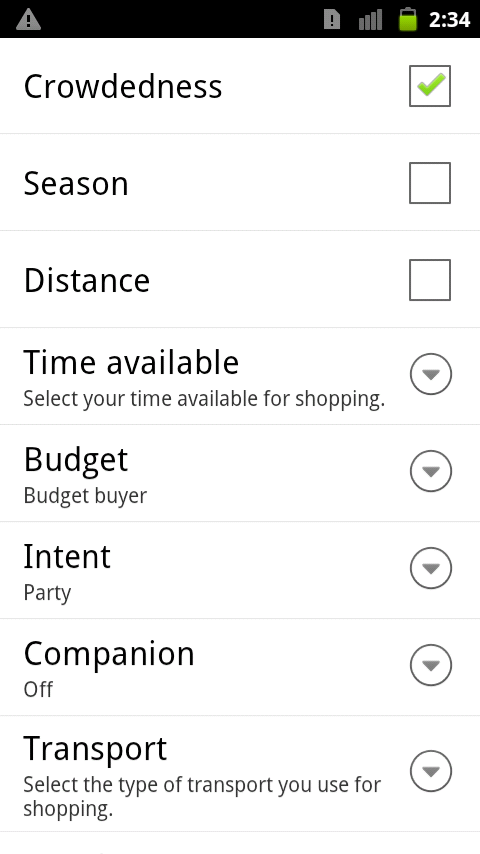
\includegraphics[height=4in]{figures/setting1.png}
  \caption{The main context settings interface.}
  \label{fig:contextSettings1}
\end{subfigure}%
\begin{subfigure}{.5\textwidth}
  \centering
  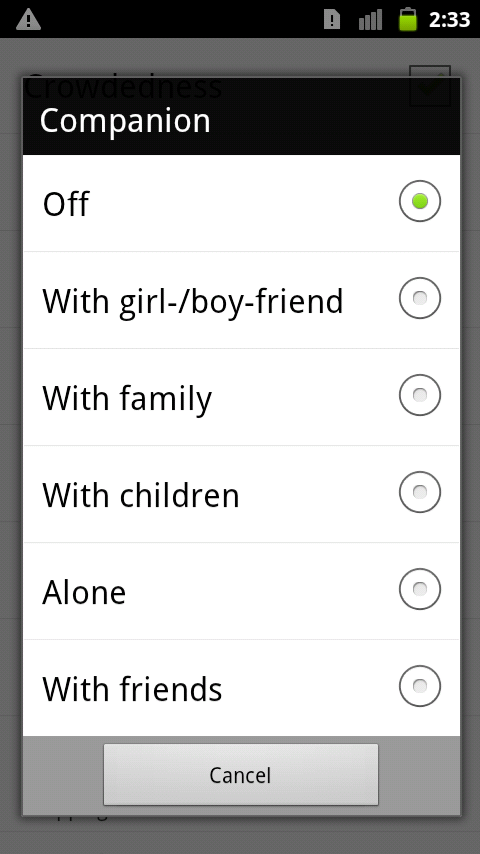
\includegraphics[height=4in]{figures/setting2.png}
  \caption{Settings dialog for condition selection.}
  \label{fig:contextSettings2}
\end{subfigure}
\caption{The final design of the context settings interface.}
\label{fig:contextSettings}
\end{figure}


After the user enables some contextual factors and provides the values for them, the system can be requested for recommendations. A short number of recommendations (nine in this thesis) will be presented to the user as depicted in Figure \ref{fig:recomm1}. If the user is interested in any of the item, she/he can click on the picture and see the detail page of the item as depicted in Figure \ref{fig:recomm2}. In the detail view, the user can see an explanation of the reason why this item is recommended to the user. It was believed that explanation can boost the transparency and user's trust in the system. A typical explanation can be "Other user bought similar clothes when they are feeling like a party animal, they are a budget buyer, it is weekend." Those are the contextual conditions that are most influential for the recommendation of the current clothes item (as was explained in previous section). 

\begin{figure}[H]
\centering
\begin{subfigure}{.5\textwidth}
  \centering
  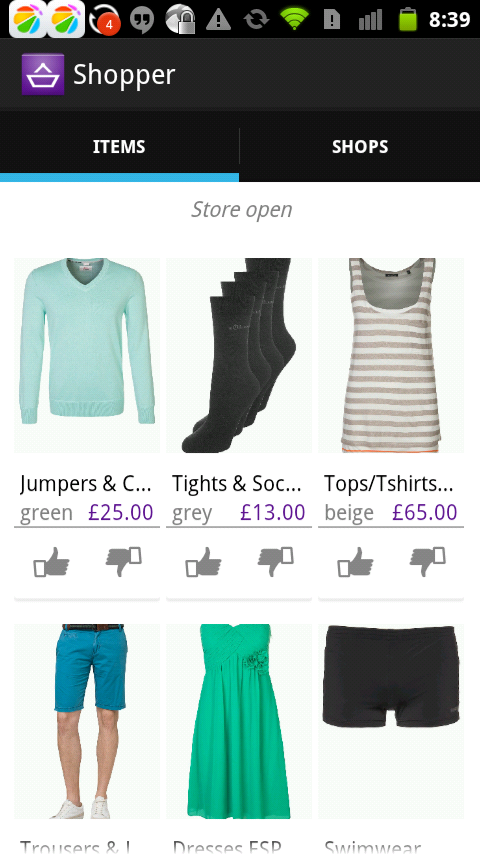
\includegraphics[height=4in]{figures/recommlist.png}
  \caption{The grid view of the recommendations in each cycle.}
  \label{fig:recomm1}
\end{subfigure}%
\begin{subfigure}{.5\textwidth}
  \centering
  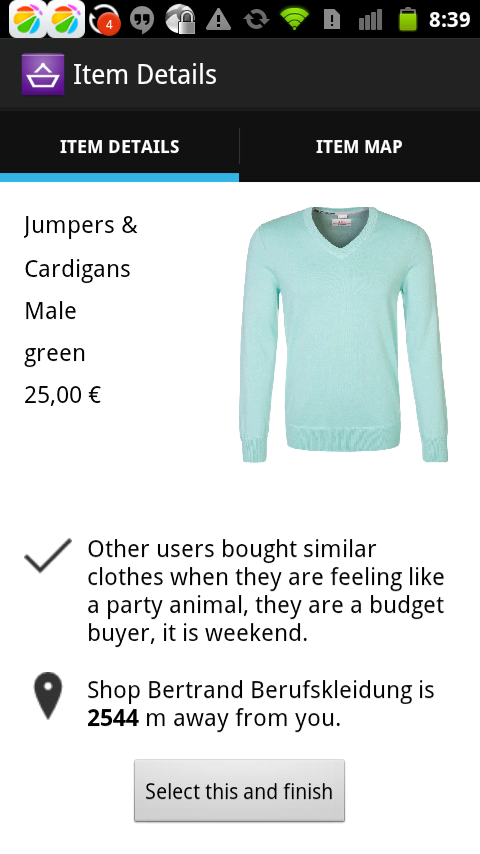
\includegraphics[height=4in]{figures/recommdetail.png}
  \caption{The detail view of each recommended item with contextual explanations.}
  \label{fig:recomm2}
\end{subfigure}
\caption{The final design of the recommendation interface.}
\label{fig:recomm}
\end{figure}

The initial consideration was to put the explanations in the main view so that they can be more directly observed by the user. However, it can be seen that there are already critiques explanations in the main view. Considering the limited space of mobile devices, the user experience will be reduced if too much text is displayed together. Moreover, each item has a different reason for being recommended. For example, if a user requests for recommendation of clothing item for context situation "budget buyer, for work and for cold temperature". One case satisfying contextual condition "budget buyer" and another case satisfying contextual condition "for work and for cold temperature" can all be recommended to the user. Thus it is better to put the explanations in the detail page of each item separately.

In the detail view, the user can also see an explanation of the location of the clothes as well as a map view of the location of the clothes relative to user's current location as depicted in Figure \ref{fig:detailmap}. For users who only want to find clothes nearby, it is an important factor for making the purchasing decision. If the user is not satisfied with the recommended clothes, she/he can critique on the item features to iteratively update the recommendations. This step corresponds to the review and iterate step in case-based recommendation as was discussed in Section \ref{sec:tcbrs}. It relies on the main functions of the system built in paper \cite{ref:30}.

\begin{figure}[H]
	\centering
	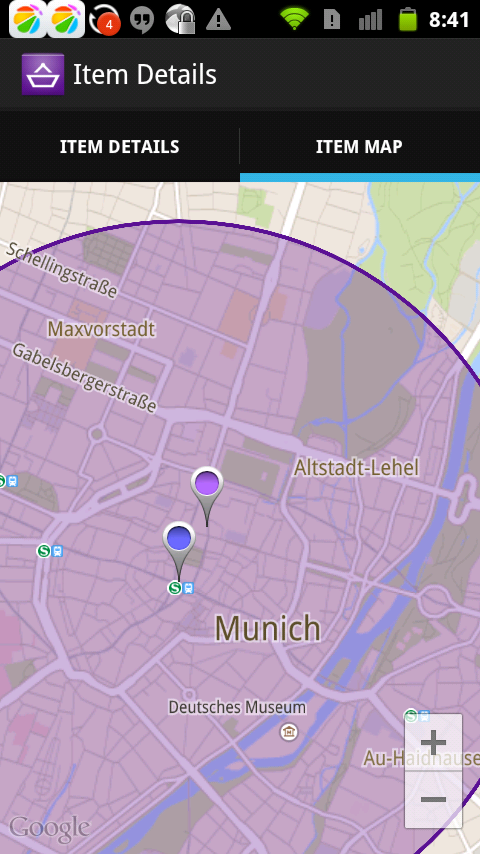
\includegraphics[height=4in]{figures/recommdetailmap.png}
	\caption{The map view in the detail view of each recommended item.}
	\label{fig:detailmap}
\end{figure}

If the user finds the ideal item, she/he can enter the detail view and click on the button "select and finish" (Figure \ref{fig:recomm2}). Then the selected item together with the current contextual situation are recorded as a new case in the system case base. 




















